\documentclass{article}
\usepackage[utf8]{inputenc}
\usepackage{amsmath}
\usepackage{amssymb}
\usepackage{graphicx}


\title{Modeling with Python and SMAP}
\author{Sarah Koehler}
\date{April 2015}

\begin{document}

\maketitle

\section{Modeling}
Many say modeling is an art. Let's look at the simplest forms of this art.

Linear Model:
\begin{align}
x(k+1) &= Ax(k) + Bu(k)  \\
y(k) &= Cx(k) + Du(k)
\end{align}
\noindent Let's assume $y(k) = x(k)$. 

In the most general case, define $x$ to be all physical \textit{outputs} and $u$ to be all \textit{controllable inputs}. You can also add an additive $ + Ed(k)$ where $d$ are all \textit{uncontrollable inputs}. 

A form that works well for Temperature dynamics is a bilinear form. Specifically:
\begin{align}
T(k+1) = AT(k) + ...
\end{align}
(TO DO: To be copied from ME 231 write ups)

\pagebreak
\section{Identification Method}
Two methods are Least Squares and Lasso. An oversimplified explanation is that Least Squares considers all data streams equally important, while Lasso selects the important streams (i.e. feature selection). Both select the corresponding weight for that stream.

Least Squares from Python scikit-learn:
\begin{figure}[h]
\centering
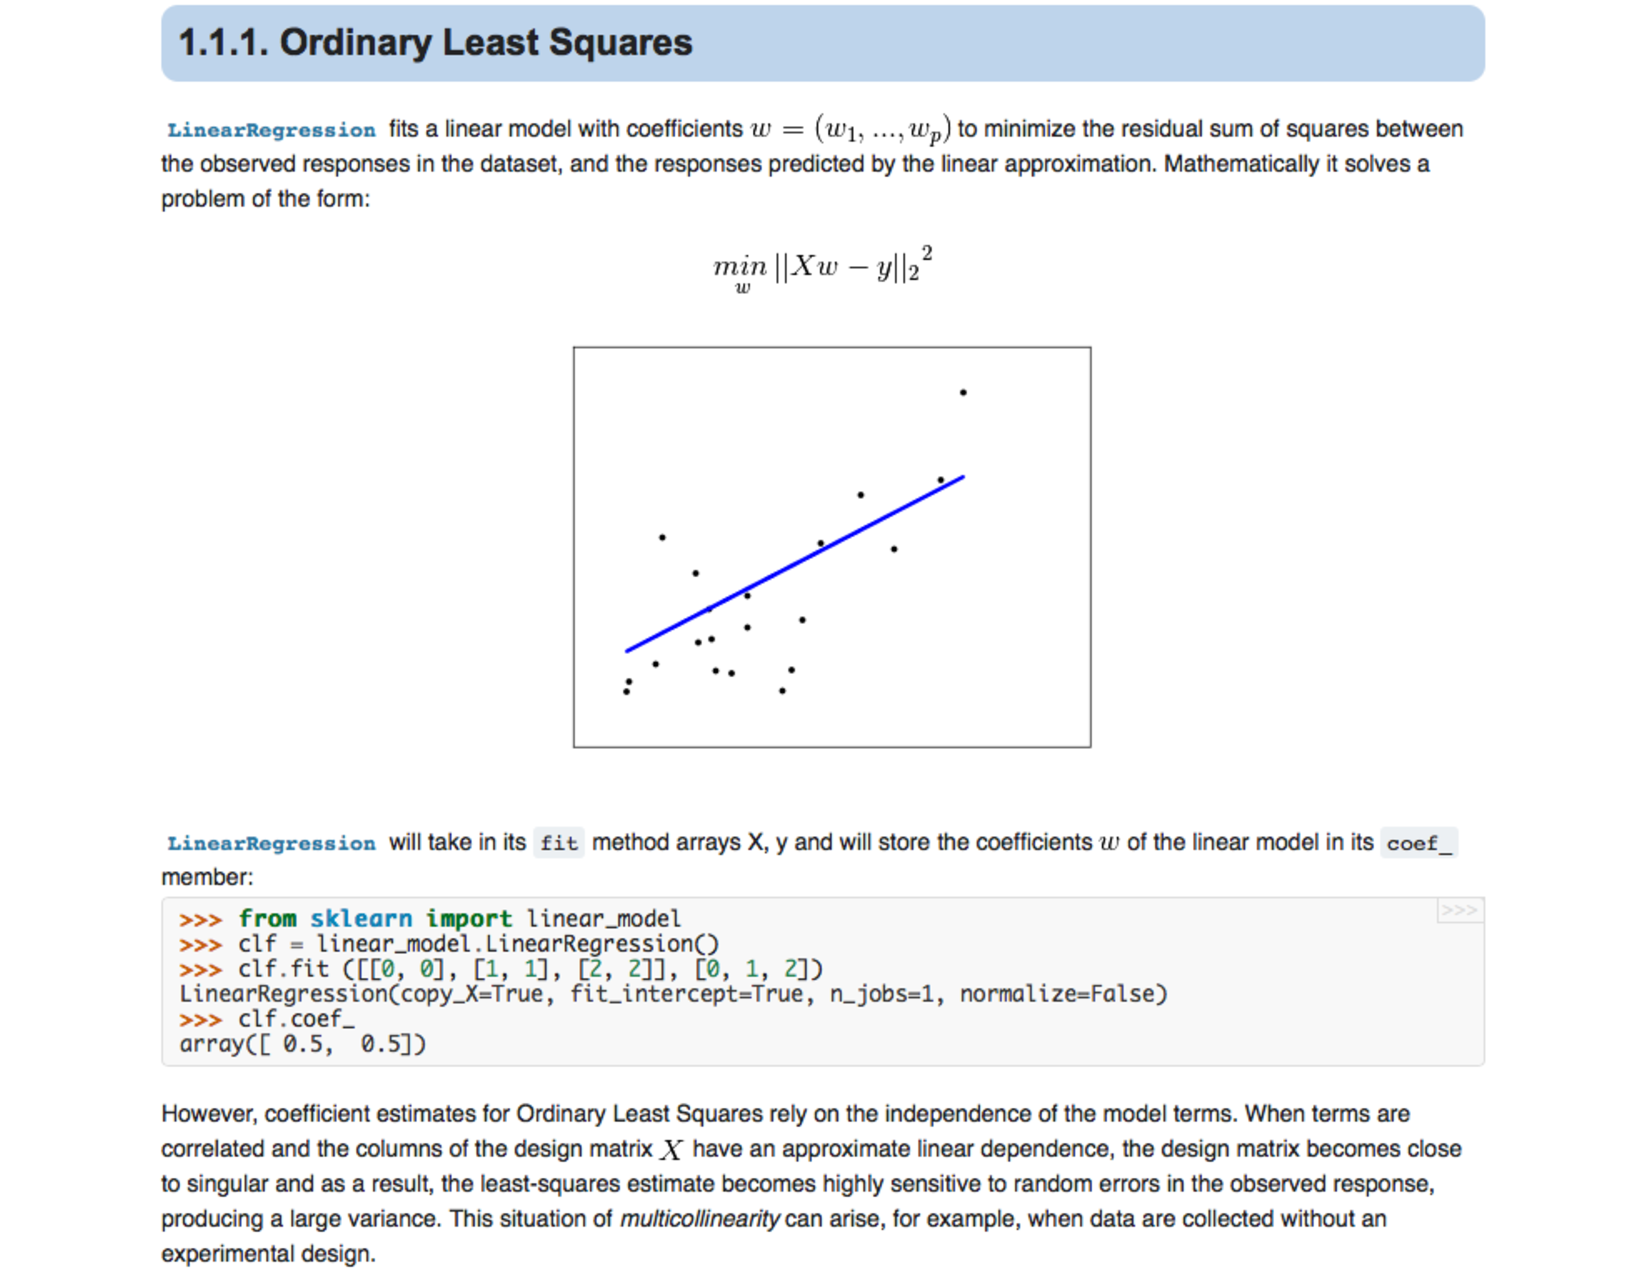
\includegraphics[width=\columnwidth]{LeastSquaresPython.pdf}
\caption{Documentation on Least Squares}
\label{fig:lasso}
\end{figure}

\pagebreak
Lasso from Python scikit-learn:
\begin{figure}[h]
\centering
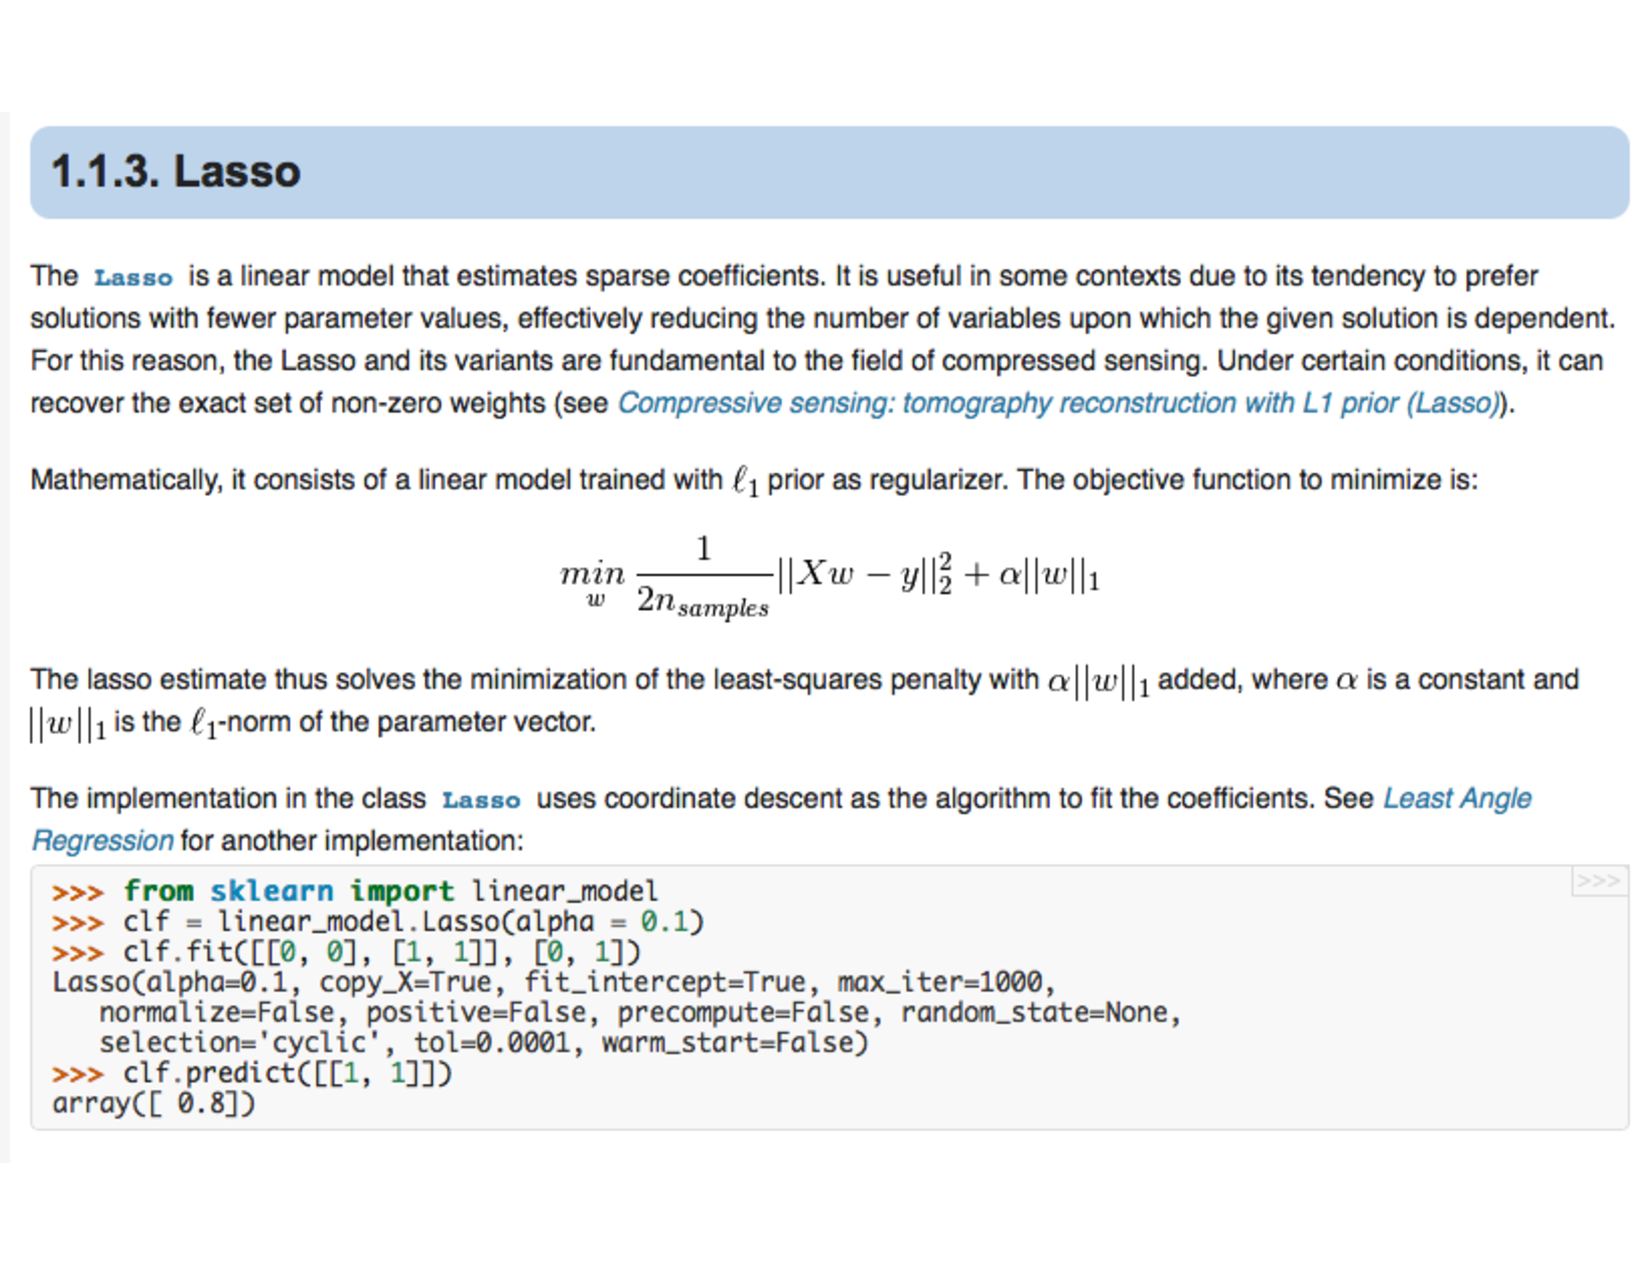
\includegraphics[width=\columnwidth]{LassoPython.pdf}
\caption{Documentation on Lasso}
\label{fig:lasso}
\end{figure}

\section{Data Manipulation}
This is the most annoying part and it would be great to never ever have to do this again.

TO DO: Copy python code when it's done and/or write the math here.

\section{Validation}
Cross-validation is important! The model usually fits the day it was identified on.

TO DO: Show some plots of same day verification and cross day verification.

\section{Matlab code}
\begin{verbatim}
% % Interpolate data
% interp_start = PDTtoUTC(datenum(2014,9,4,4,0,0));
% interp_end = PDTtoUTC(datenum(2014,9,4,16,0,0));
interp_start = datenum(2014,8,30,10,1,0);
interp_end = datenum(2014,8,30,16,0,0);
interp_times = (interp_start:1/24/60:interp_end)';


fan_interp = interp1(fan_data(:,1),fan_data(:,2),interp_times);
temp_interp = interp1(temp_data(:,1),temp_data(:,2),interp_times);
supplytemp_interp = interp1(supplytemp_data(:,1),supplytemp_data(:,2),interp_times);

% Solve least squares using quadprog
N = length(interp_times)-2;
H = 2*(blkdiag(zeros(2,2),eye(N)));
f = zeros(N+2,1);
Aeq = [zeros(N,2),-eye(N)];
beq = zeros(N,1);
for k = 1:N
   f(k+2) = -2*temp_interp(k+1);
   Aeq(k,1:2) = [-fan_interp(k)*temp_interp(k),fan_interp(k)*supplytemp_interp(k)];
   beq(k) = -temp_interp(k);
end

% options = optimset('Algorithm','interior-point-convex');
% [x,cost] = quadprog(H,f,[],[],Aeq,beq,[],[],[],options);
[x,cost] = quadprog(H,f,[],[],Aeq,beq);

a = x(1);
b = x(2);

%% Least Squares via A\b
A = Aeq(:,1:2);
b = zeros(N,1);
for k = 1:N
   b(k) = -temp_interp(k)+temp_interp(k+1);
end

x = A\b;
a = x(1);
b = x(2);

\end{verbatim}

\section{Python code}
At this point can open up Python code like Arka did and expose the issues we have with its structure.

TO DO: Can also make a list of issues here:
\begin{itemize}
\item Cannot choose system ID procedure without digging into code
\item Need a library of models to choose from? Not everything is linear or bilinear...
\end{itemize}

\end{document}
